%!TEX root = /Users/simo/Documents/PFC/memoria/memoria.tex
\section{Dibujo} % (fold)
\label{sec:javascript_dibujo}
La situación actual es de la disposición de una serie de funciones con las que generar gráficos vectoriales y modificarlos, funcionando en la gran mayoría de navegadores. Proceder a implementar unas herramientas de dibujo mediante esta librería es ahora posible. En esta sección no se pretende describir el proceso de creación de una herramienta de dibujo genérica, sino las peculiaridades de Javascript respecto a la forma en que trata los eventos, las diferencias entre navegadores, y la influencia de la estructura del documento (HTML y CSS).

El reto con el que uno se enfrenta inicialmente es el de conseguir capturar los eventos de ratón de forma adecuada. En los usos típicos de las herramientas deseadas, y exceptuando la introducción de texto, toda la interacción se hace mediante el ratón. Hay que recordar también el entorno en el que estas acciones se ejecutarán: habrá un marco en la página web (un elemento DIV) dentro de el cual se podrá dibujar, y una serie de elementos externos a este marco. Esto es importante puesto que es posible que los elementos exteriores interfieran de alguna forma. Dichos elementos exteriores deberán ser los siguientes:

\begin{description}
  \item[Elementos estáticos] El nombre del documento, el link de vuelta a la web \emph{normal}, así como cualquier otro elemento estático.
  \item[Barra de herramientas] Debe haber alguna forma, lo más sencilla posible, de elegir las herramientas a usar, y de configurarlas (elegir el color, grosor y transparencia). Estos elementos pueden complicar más la tarea pues deben ser dinámicos, y controlar también eventos de ratón y/o teclado.
  \item[Lista de usuarios] Esta lista deberá ser dinámica también, puesto que los usuarios podrán entrar y salir de la pizarra, y deberá informarse al resto de usuarios activos de alguna forma. No influirá con el ratón, pero si ejecutará operaciones periódicamente, y ejercerá cambios sobre el código de la página, si bien no sobre la pizarra en si.  
  \item[Selector de páginas] De la misma forma que la lista de usuarios, éste influirá poco en cuanto a eventos se refiere, pero será actualizado dinámicamente, y debe permitir flexibilidad por si el usuario no tiene permiso para cambiar de página.
\end{description}

En este momento, para dibujar, es solo necesario considerar la barra de herramientas. Más adelante, cuando se implementen más funciones, se deberá considerar cómo implementarlas, y de qué forma influencian a lo que ya se tiene.

\subsection{Barra de herramientas} % (fold)
\label{sub:barra_de_herramientas}

La opción de selección de herramientas es relativamente sencilla, puesto que solo necesita detectar cuando se clica en el elemento representativo de la herramienta y defina que esa es la herramienta activa. En javascript existen dos formas básicas de capturar eventos. La primera es utilizando el propio código HTML, con una línea como la siguiente:
\begin{Verbatim}[commandchars=@\[\]]
  @PYba[<div] @PYaQ[id=]@PYad["line-tool"] @PYaQ[onClick=]@PYad["setTool('line');"]@PYba[>]Línea@PYba[</div>]
\end{Verbatim}

%\begin{verbatim}
%  <div id="line-tool" onClick="setTool('line');">Línea</div>
%\end{verbatim}
Todos los navegadores entienden estas definiciones, aunque no se consideran elegantes, y son bastante restrictivas por diversas razones.

Una segunda manera sería, mediante jQuery, con una línea como la siguiente (suponiendo que se quiere definir la herramienta línea al hacer click sobre el elemento con id \texttt{line-tool}):
\begin{Verbatim}[commandchars=@\[\]]
  $(@PYaX["#line-tool"]).bind(@PYaX["click"]@PYbf[,] @PYbh[function](){setTool(@PYbe['line']);});
\end{Verbatim}

%\begin{verbatim}
%  $("#line-tool").bind("click", function(){setTool('line');});
%\end{verbatim}
Aunque aparentemente pueda parecer más complicada, es mucho más limpia en cuanto a que se separa lo que es el contenido de la web (HTML) con lo que es su comportamiento, de la misma forma que se separa su diseño utilizando CSS, y se considera poco elegante y práctico añadir estilos directamente en el código de los elementos.

En cuanto al problema de la configuración de las herramientas, existen múltiples y variadas soluciones. No es posible encontrar de forma nativa una manera de seleccionar un color, o de tener una barra de desplazamiento. Las únicas herramientas de las que se dispone en HTML para introducción de datos, son campos de texto o listas. Esto, aunque suficiente, es poco útil para el usuario, pues es más sencillo seleccionar un color de una paleta de colores que escribiendo su código RGB. De la misma forma, es más intuitivo usar una barra de desplazamiento para elegir el grosor o la transparencia, que escribiendo sus valores directamente. En otro tipo de herramientas sería interesante poder hacer estas cosas a mano, si se necesitara de más precisión, pero en esta aplicación es más prioritaria la agilidad de uso.

A pesar de no existir nada directamente en HTML, existen múltiples opciones que, mediante javascript, simulan estos elementos.

\subsubsection{Colores} % (fold)
\label{ssub:colores}
Para esta opción se ha decidido crear un mini-panel con ocho posibles colores, en vez de tener un selector de colores completo como los típicos de los programas de dibujo. No se cree necesario elegir una grandísima variedad de colores y con mucha precisión, sino ofrecer una pequeña cantidad de colores muy diferentes, vivos y fácilmente identificables.

\begin{figure}[h!]
\centering
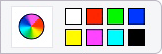
\includegraphics{color_selector.png}
\caption{Selector de colores}\label{fig:color_selector}
\end{figure}

El código para este selector es extremadamente sencillo y no consta más que de elementos sobre los que clicar para seleccionar el color, de la misma forma que se escogen herramientas.
% subsubsection colores (end) 

\subsubsection{Grosor y transparencia} % (fold)
\label{ssub:grosor_y_transparencia}
Mediante jQuery UI \footnote{jQuery UI - \url{http://ui.jquery.com/}}, una extensión a jQuery, es posible generar los llamados Sliders. Con un par de líneas de código se puede generar un Slider que permita seleccionar un valor de entre un rango, y que ejecute código personalizado al mover la manilla y al soltarla:
\begin{Verbatim}[commandchars=@\[\]]
  $(@PYaX["#fill-dialog"]).slider({min@PYbf[:] @PYag[20]@PYbf[,] max@PYbf[:]@PYag[100]@PYbf[,] startValue@PYbf[:] @PYag[80]@PYbf[,] change@PYbf[:] @PYbh[function](e@PYbf[,]ui){
    fill @PYbf[=] (ui.value@PYbf[/]@PYag[100]);
  }@PYbf[,] slide@PYbf[:] @PYbh[function](e@PYbf[,]ui){
    $(@PYaX["#fill"]).html(ui.value);
  }});
\end{Verbatim}

%\begin{verbatim}
%  $("#fill-dialog").slider({min: 20, max:100, startValue: 80, change: function(e,ui){
%    fill = (ui.value/100);
%  }, slide: function(e,ui){
%    $("#fill").html(ui.value);
%  }});
%\end{verbatim}

Esta función crea un slider en el elemento con id \texttt{\#fill-dialog}, con posibles valores entre el 20 y el 100, puesto de forma predefinida a 80, que al cambiar actualiza el contenido del elemento con id \texttt{\#fill} (campo de texto mostrando el valor actual), y que al soltarse actualiza la variable \texttt{fill} con el valor seleccionado.

\begin{figure}[h!]
\centering
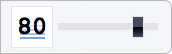
\includegraphics{fill_selector.png}
\caption{Slider selector de relleno (transparencia)}\label{fig:fill_selector}
\end{figure}

En la figura \ref{fig:herramientas} se puede observar el resultado final, con las tres últimas ocultas, puesto que aparecen al pasar el ratón por encima.

\begin{figure}[h!]
\centering
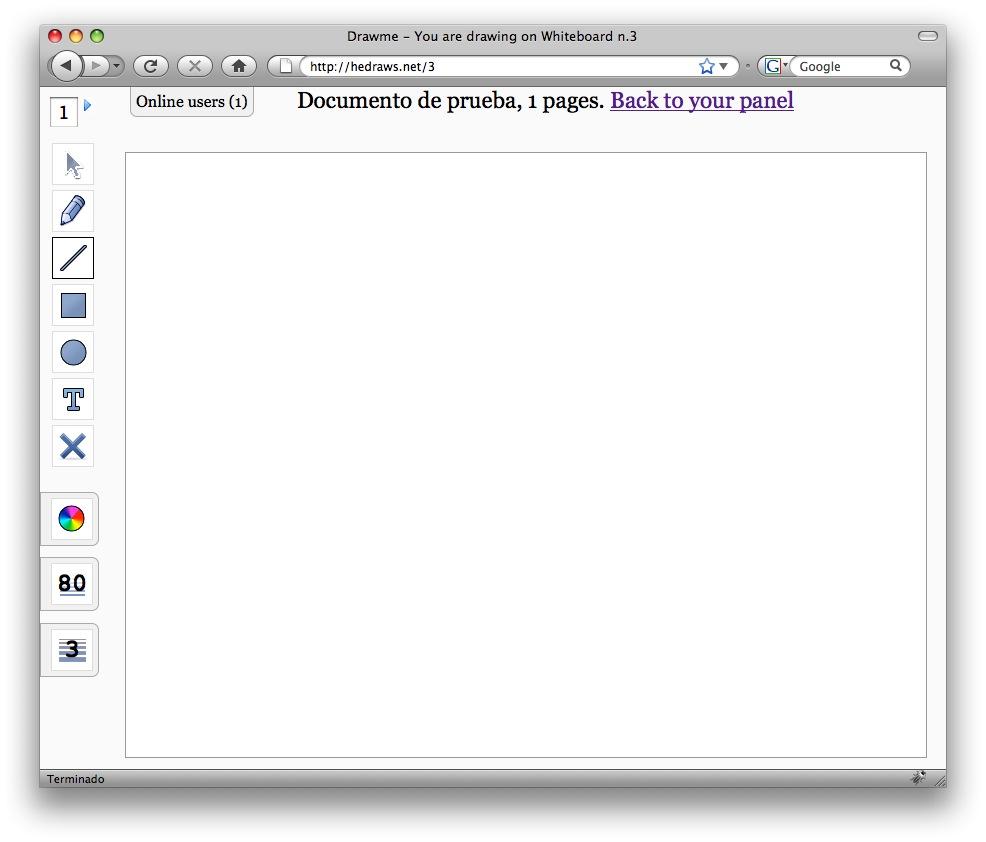
\includegraphics[totalheight=0.6\textheight]{resultadofinal.jpg}
\caption{Barra de herramientas final}\label{fig:herramientas}
\end{figure}

% subsubsection grosor_y_transparencia (end)


% subsection barra_de_herramientas (end)

\subsection{Eventos de ratón} % (fold)
\label{sub:eventos_de_raton}

Los tres eventos básicos de un ratón son los de pulsar un botón (\texttt{mousedown}), moverse (\texttt{mousemove}) y soltar el botón (\texttt{mouseup}). Los tres son necesarios, puesto que son, en ese orden, cuando se empieza a dibujar un elemento, cuando se va modificando, y cuando finalmente se \emph{suelta}, quedando gravado definitivamente hasta que es borrado (a excepción del texto, que es un tanto más peculiar, y se explica en otro apartado).

El que solo se quiera poder dibujar dentro del marco seleccionado para ello, hace que se planteen una serie de problemas.

\begin{itemize}
  \item Cuando se empieza a dibujar dentro del marco, pero se mueve el ratón fuera de él.
  \item Cuando se suelta el botón fuera del marco.
  \item O peor aún, cuando se suelta el botón fuera de la ventana.
\end{itemize}

\subsubsection{¿Cómo funcionan los eventos en Javascript?} % (fold)
\label{ssub:como_funcionan_los_eventos}

En Javascript es posible capturar eventos en cualquier elemento, y siempre sucederá de forma jerárquica según la visibilidad que se tiene de los distintos elementos. Es decir, si se tiene un trozo de código como el siguiente:
\begin{Verbatim}[commandchars=@\[\]]
  @PYba[<div]@PYba[>]
    @PYba[<p]@PYba[>]Hola @PYba[<a] @PYaQ[id=]@PYad["albert-link"] @PYaQ[href=]@PYad["/users/albert"]@PYba[>]Albert@PYba[</a>], qué tal estás?@PYba[</p>]
  @PYba[</div>]
\end{Verbatim}

%\begin{verbatim}
%  <div>
%    <p>Hola <a id="albert-link" href="/users/albert">Albert</a>, qué tal estás?</p>
%  </div>
%\end{verbatim}

y se hace click en la palabra Albert, saltará un evento en el elemento \texttt{a}, cuando acabe de hacer lo que sea que debe hacer, y pasará a ejecutar el evento del elemento \texttt{p}, seguirá con el del \texttt{div}, y acabará con el del elemento \texttt{body}, que en cada documento HTML es el contenedor de todo lo que se ve en pantalla. Por tanto, si se quisiera capturar cualquier movimiento de ratón en la pantalla, se deberían capturar los eventos \texttt{mousemove} del elemento \texttt{body}.

Por otro lado, el ejemplo anterior tiene un problema, y es que el evento \texttt{click} de todo elemento \texttt{a} lo que hace es mandar al usuario a la página que éste linca. En caso de querer, por ejemplo, en vez de mandar al usuario a la página con los detalles personales de Albert, que está en \texttt{/users/albert}, si no que queremos hacerlo más dinámico y mostrarlo directamente mediante Javascript, se debería capturar el evento click de dicho elemento, y realizar lo necesario (una llamada por ajax, creación o modificación de otro elemento para mostrar la información, etc). Pero el comportamiento de los eventos en Javascript, por defecto, al acabar de atender el evento capturado por el usuario, sigue ejecutando el comportamiento normal de dicho elemento (ir a la página enlazada), a menos que la función ejecutada devuelva un valor falso.

Es decir, el código javascript debería ser semejante al siguiente:
\begin{Verbatim}[commandchars=@\[\]]
  $(@PYaX["#albert-link"]).bind(@PYaX["click"]@PYbf[,]@PYbh[function](){
    @PYaE[// Obtener información y mostrarla dinámicamente]
    . . .
    @PYaz[return] @PYbd[false]@PYbf[;]
  });
\end{Verbatim}

%\begin{verbatim}
%  $("#albert-link").bind("click",function(){
%    // Obtener información y mostrarla dinámicamente
%    . . .
%    return false;
%  });
%\end{verbatim}

Esto es considerado una buena técnica puesto que en caso de estar ante un usuario sin soporte para Javascript, el sistema mostrará la información de todas maneras, aunque no de una forma tan dinámica. En el caso que interesa a este proyecto, hay que comprender este comportamiento para que, por ejemplo, se pueda seguir dibujando aun estando fuera del marco, o para tener varias cosas que estén encima del marco, poder trabajar con ellas mediante eventos, y que éstos no influyan al proceso de dibujo.

% subsubsection como_funcionan_los_eventos (end)

\subsubsection{¿Cómo capturarlos?} % (fold)
\label{ssub:como_capturarlos}

En este caso, por el comportamiento que se le quiere dar a la aplicación, es necesario estar siempre al tanto de los siguientes eventos:
\begin{itemize}
  \item Cuando se pulsa un botón del ratón dentro del marco. Si se pulsa el ratón fuera del marco, no debe afectar al dibujo, más que en el caso de las herramientas o el selector de páginas, pero estos trabajan de forma independiente.
  \item Se debe saber en todo momento cuándo se está moviendo el ratón, y cuándo se suelta el botón, debido a los casos explicados anteriormente, si va dibujando hasta soltar el ratón fuera del marco, o de la ventana. Si se ignoraran los eventos fuera del marco, se producirían comportamientos incómodos, como que se deje de mover una línea por rozar un borde, o que, al no enterarse de que se ha soltado el botón, se siga dibujando aún cuando no se está pulsando.
\end{itemize}

Sabiendo, como se ha comentado antes, que siempre se tendrá un elemento con id \texttt{\#container}, que será el \texttt{marco}, el código para capturar los eventos es el siguiente:

\begin{Verbatim}[commandchars=@\[\]]
  $(@PYaY[document]).ready(@PYbh[function](){
    $(container).bind(@PYaX["mousedown"]@PYbf[,] mouseDown);
    $(@PYaX["body"]).bind(@PYaX["mousemove"]@PYbf[,] mouseMove);
    $(@PYaX["body"]).bind(@PYaX["mouseup"]@PYbf[,] mouseUp);
  });
\end{Verbatim}

%\begin{verbatim}
%  $(document).ready(function(){
%    $(container).bind("mousedown", mouseDown);
%    $("body").bind("mousemove", mouseMove);
%    $("body").bind("mouseup", mouseUp);
%  });
%\end{verbatim}

En este caso, en vez de implementar las tres funciones directamente, se pasan como parámetro. Puesto que Javascript entiende las funciones también como objetos, es posible definirlas con anterioridad de la misma forma que se definiría una variable, para luego usarla como parámetro. jQuery automáticamente pasa a estas funciones la \textbf{variable de evento}, que es un descriptor del entorno en que ha sucedido el evento. Cosas como la posición del ratón, el elemento al que se estaba apuntando, qué botón se ha pulsado, se pueden consultar en este objeto.

% subsubsection _cómo_capturarlos_ (end)

\subsubsection{¿Dónde está el ratón?} % (fold)
\label{ssub:donde_esta_el_raton}

No hay que olvidar, que lo que se está haciendo es, en cierta medida, \emph{incrustar} un elemento SVG, o un conjunto de elementos VML, dentro de otro elemento DIV. A la hora de crear elementos, por tanto, es necesario especificar las posiciones como pixels respecto del inicio del marco. Mediante jQuery es posible obtener la posición absoluta del ratón, respecto del total de la ventana del navegador, pero para este caso es necesario algo más preciso, que tenga en cuenta también la posición del DIV, y o si se ha hecho scroll o no.

Los atributos que se pueden consultar mediante la \textbf{variable de estado} (\texttt{event} a partir de ahora) del evento, y el resto del DOM, y que son útiles para posicionar elementos, son las siguientes.

\begin{description}
  \item[\texttt{event.clientX} y \texttt{event.clientY}] Estos atributos devuelven la posición del ratón respecto a lo que ahora se ve en el navegador. Esto quiere decir, aunque se haya hecho scroll, si se clica en la esquina superior izquierda, ambos valdrán 0.
  \item[\texttt{container.offsetLeft} y \texttt{container.offsetTop}] Recordando que \texttt{container} es el DIV contenedor dentro del cual se anidarán los elementos, estos dos atributos devuelven su posición respecto a los bordes absolutos de la página, ignorando si se ha hecho scroll o no.
  \item[\texttt{document.body.scrollLeft document.body.scrollTop window.pageXOffset window.pageYOffset}] Este es un claro ejemplo de las diferencias comentadas entre el DOM ofrecido por diferentes navegadores, y que generalmente jQuery ayudaría a resolver. Los dos primeros funcionarían en \texttt{IE}, y devuelven la cantidad de pixels que se ha hecho scroll, tanto lateral como verticalmente, y los segundos son sus equivalentes para todo el resto de navegadores.
\end{description}


\begin{figure}[h!]
\centering
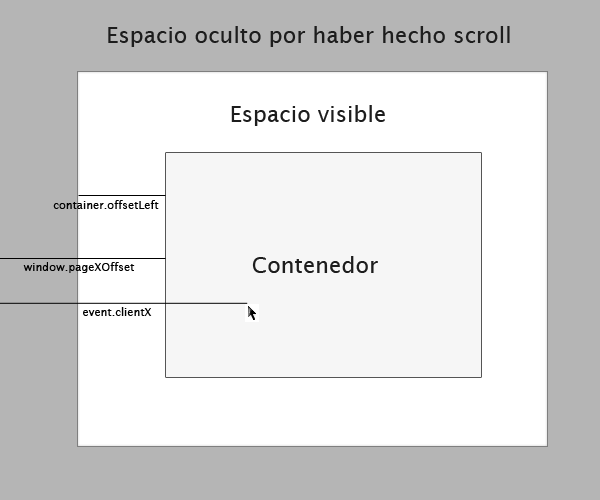
\includegraphics[width=\textwidth]{mouse_pointer.png}
\caption{Esquema de distancias de los distintos elementos}\label{fig:mouse_pointer}
\end{figure}

La figura \ref{fig:mouse_pointer} muestra un pequeño esquema de estas distancias. Mediante estos tres tipos atributos es posible averiguar la posición del ratón respecto al DIV contenedor, sea cual sea la situación de la página, con estas instrucciones.

\begin{Verbatim}[commandchars=@\[\]]
@PYaE[//IE]
x @PYbf[=] e.clientX @PYbf[-] container.offsetLeft @PYbf[+] @PYaY[document].body.scrollLeft@PYbf[;]
y @PYbf[=] e.clientY @PYbf[-] container.offsetTop @PYbf[+] @PYaY[document].body.scrollTop@PYbf[;]
@PYaE[//RESTO]
x @PYbf[=] e.clientX @PYbf[-] container.offsetLeft @PYbf[+] @PYaY[window].pageXOffset@PYbf[;]
y @PYbf[=] e.clientY @PYbf[-] container.offsetTop @PYbf[+] @PYaY[window].pageYOffset@PYbf[;]
\end{Verbatim}

%\begin{verbatim}
%//IE
%x = e.clientX - container.offsetLeft + document.body.scrollLeft;
%y = e.clientY - container.offsetTop + document.body.scrollTop;
%//RESTO
%x = e.clientX - container.offsetLeft + window.pageXOffset;
%y = e.clientY - container.offsetTop + window.pageYOffset;
%\end{verbatim}

Con estos conocimientos ya es posible programar las herramientas de línea, trazo de lápiz, elipse y caja, que son la base de lo que este proyecto pretendía. El resto del trabajo necesario para programar estas herramientas es de puesta en práctica de estos apartados, y no se considera importante destacar nada más. El código de la implementación se puede encontrar en el anexo.

% subsubsection donde_esta_el_raton (end)

% subsection eventos_de_ratón (end)

\subsection{Introducción de texto} % (fold)
\label{sub:introduccion_de_texto}

El método tradicional para introducir texto en páginas web, es mediante los elementos de formulario \texttt{input} de tipo \texttt{text} o los llamados \texttt{textarea}. Para esta situación el más adecuado será el \texttt{textarea} puesto que el otro es simplemente una línea, y los \texttt{textarea} se pueden redimensionar a voluntad.

El efecto que se quiere lograr es el de crear un pequeño recuadro donde escribir, y al hacer click fuera o pulsar tabulador, este texto pase a formar parte del documento. Existe un requisito importante, y es que la posición del texto mientras se escribe, y cuando se introduzca \emph{definitivamente}, debe ser la misma, para así no confundir al usuario.

Este proceso difiere del resto de herramientas por necesitar de dos pasos distintos, uno para crear un \texttt{textarea} en alguna posición, y otro para acabar agregándolo finalmente.

\subsubsection{Generación de un textarea} % (fold)
\label{ssub:generacion_de_un_textarea}
En este caso, la creación del elemento no será en el evento \texttt{mousedown}, puesto que los usuarios están acostumbrados que las cosas suceden al soltar el botón del ratón, no al pulsarlo. Al detectar un evento de tipo \texttt{mouseup} con la herramienta de texto seleccionada, y siempre y cuando se haya clicado antes dentro del contenedor, se crea dinámicamente este textarea, posicionado mediante CSS con origen en la posición del ratón.

% subsubsection generación_de_un_textarea (end)

\subsubsection{Introducción del texto} % (fold)
\label{ssub:introduccion_del_texto}
Para poder averiguar cuando el usuario quiere dejar de escribir e introducir el texto en el documento, hay que simular de alguna manera las distintas posibilidades por las que un usuario puede pretender hacer esto. Lo más intuitivo es que esto suceda cuando el elemento pierda el \texttt{focus}, es decir, cuando se clique fuera o se pulse tabulador. La forma de asegurarse que esto sucede es capturando los eventos \texttt{change} y \texttt{blur}, además de mediante los eventos que ya se capturan de mousedown y mouseup.

Al detectar este suceso, se genera un nuevo DIV, que estará anidado dentro de del contenedor igual que el resto de elementos, y posicionado mediante CSS en el mismo lugar en el que estaba el \texttt{textarea}, con la misma fuente, tamaño y color.


% subsubsection introducción_del_texto (end)

% subsection introducción_de_texto (end)

\subsection{Goma de borrar} % (fold)
\label{sub:goma_de_borrar}

Existen dos vertientes diferentes a la hora de plantear la goma de borrar. La funcionalidad típica a la que se está acostumbrado en los programas de dibujo, es a la de una goma que, de forma inversa a lo que sería el lápiz, borra solamente el trozo por el que se pasa por encima. Esta vertiente, por el tipo de datos con los que se está trabajando, sería extremadamente difícil de implementar, pues al pasar por en medio de un elemento, se debería detectar en qué punto ha pasado, y dividir los elementos en múltiples trazos (si son líneas o trazos de lápiz), o prácticamente imposible de representar si se tratara de una caja o una elipse.

La otra vertiente, más usada en los programas de pizarra compartida por la sencillez, tanto para el programador, como para el usuario, es la una goma de borrar que no elimina solo aquellas zonas por las que pasa, sino que elimina el elemento entero. Situándose en la posición del usuario que está utilizando esta pizarra para acompañar sus explicaciones, la situación clásica es la de estar resaltando distintos elementos de la página, que luego querrá eliminar para seguir su explicación. Tener la facilidad de clicar en el elemento, y que este desaparezca por completo, sería muy práctico, y posiblemente la mejor solución.

Existen múltiples formas de enfocar este problema, puesto que es posible capturar eventos del ratón en cualquiera de los elementos que se generan, no solamente en el contenedor. Sin embargo, se considera que esto es excesivamente complejo, y que gracias al atributo \texttt{target} de la \textbf{variable de estado} del evento, es posible solucionar todos los problemas con los eventos que ya se capturaban con anterioridad.

Suponiendo que se tiene la herramienta de goma de borrar seleccionada, y que se quiere borrar algo que está en un punto donde coincide, por ejemplo, un círculo y una línea. El círculo se ha dibujado después de la línea, por lo tanto está por encima, así que lo más lógico es que se borrara primero. Al hacer click, el evento se generará en el elemento círculo, pues es el que está visible en ese momento, pero tal y como se ha explicado en la sección \textbf{¿Cómo capturarlos? }\ref{ssub:como_capturarlos}, este evento irá saltando de superior al inferior, llegando, en efecto, a los eventos que se capturan en el contenedor o en la etiqueta \texttt{body}.

Una vez más, mediante la \texttt{variable de estado} es muy fácil saber cuál fue el objeto que generó el evento originalmente, a pesar de que en ese momento se esté tratando el evento de un elemento \emph{inferior}. Y una vez más, existe un conflicto entre los atributos generados por \texttt{IE}, y los atributos generados por el resto de navegadores.

\begin{verbatim}
// IE
event.srcElement
// SVG
event.target
\end{verbatim}

% subsection goma_de_borrar (end)

% section javascript_dibujo (end)